\chapter{Mögliche Soll-Situation im Hinblick auf die heutigen und zukünftigen Aufgaben - AE, JL, HS}
\label{chapter_sollsituation_INM}
\textit{Autoren: Andreas Ebling, Julia Lübke, Hannes Sprafke}

Eine mögliche Soll-Situation für das Informationsmanagement an der Hochschule Emden/Leer baut auf der Ist-Situation auf, und berücksichtigt die allgemeinen Grundlagen, Besonderheiten von Hochschulen, Trends und Best Practices zum Thema. Wichtige Aspekte an einer kleinen Hochschule sind, neben der großen Autonomie der Beteiligten, auch deren Heterogenität als Gruppe, und die relative Beschränktheit von Ressourcen.

Es werden im folgenden Kapitel also zunächst konzeptionell die Rahmenbedingungen eines möglichen Informationsmanagements hinsichtlich des Endergebnisses betrachtet, sowie die Formalisierung eines Entwicklungsprozesses, der von den Bedingungen der Hochschule profitiert. Im weiteren werden zu diesem Zweck geeignete IT-Systeme betrachtet, sowie erörtert, in welchem personellen Rahmen die Konzeption unter den spezifischen Bedingungen der Hochschule sinnvoll unterzubringen ist.

\section{Marketing - AE}
\label{section_marketing}
Das Marketing hat neben dem typischen Aufgabenbereich der Außenrepräsentation durch die Besonderheiten einer Hochschule auch einen Aufgabenbereich der Innenrepräsentation. Im folgenden werden diese Bereiche getrennt betrachtet.

\subsection{Externes Hochschulmarketing}
\label{subsection_externes_hochschulemarketing}
Das externe Marketing der Hochschule bezieht sich auf die klassischen Marketingaufgaben, das Produkt und die Marke vorteilhaft darzustellen. Im Falle einer Hochschule ist dies die attraktive Darstellung gegenüber zukünftigen Studierenden, Forschungsinteressierten und Geldgebern.

\subsubsection{Webseite}
Zentrales Element bleibt die Hochschulwebseite, die mit aktuellen, offenen Möglichkeiten von HTML 5, CSS 3 und JavaScript den Funktionsumfang einer App erreichen kann, ohne auf spezielle oder spezifische Spezialtechnologien zu setzen. Besonders sei an dieser Stelle die Möglichkeit genannt, mittels Media Queries in CSS Größen und Darstellungsmöglichkeiten von Endgeräten unabhängig von konkreten Betriebssystemen und Hardwareplattformen abzudecken.\footnote{vgl. \cite{w3c_media_queries_url}}

Dies ist vor dem Hintergrund wichtig, dass beispielsweise eine native App für iPhones zwingend durch den Appstore der Firma Apple installiert werden muss\footnote{vgl. \cite{apple_app_distribution_guide_url}}, dessen Nutzungsbedingungen sich für die Hochschule in Form von Kosten oder Inhaltseinschränkungen zu Ungunsten der Hochschule verändern könnten. Mit einer nativen App lässt sich trotzdem nur ein beschränkter Nutzerkreis ansprechen, da mehrere Betriebssysteme und Versionen verbreitet sind.\footnote{vgl. \cite{kantarworldpanel_mobile_betriebssysteme_url}} Sollen mehrere Apps für verschiedene Plattformen gepflegt werden, so ist dies mit zusätzlichen Aufwand, und damit Bindung von Ressourcen verbunden.

Eine Neuauflage der Hochschulwebseite mit aktuellen Möglichkeiten und per CSS an verschiedene Darstellungsgrößen angepasst erreicht dagegen jedes internetfähige Gerät mit Browser. Sollte ein neuer Formfaktor wichtig werden, zum Beispiel der einer Smartwatch, so lässt sich dies über eine Erweiterung des Stylesheets erreichen, ohne eine komplette Neuentwicklung in Auftrag zu geben.

\subsubsection{Soziale Netzwerke}
Soziale Netzwerke wie facebook oder twitter sind nicht eindeutig zu bewerten. Auftritte auf diesen Plattformen können nicht alleine stehen, da nicht jeder einen Account bei einem sozialen Netzwerk hat, benötigen aber durch ständigen Nutzerkontakt eigenständige Pflege und Aufsicht, was an einer kleinen Hochschule Personal bindet.

Für interne Kommunikation und Daten ist ein kommerzielles soziales Netzwerk nicht geeignet, da AGB und Nutzungsbedingungen des Netzwerks mit deutschen Datenschutz- und Urheberrechtsvorgaben, die für eine deutsche Hochschule gelten, in Konflikt stehen können. Auch hier sind Nutzer zu berücksichtigen, die kein Interesse haben, einen Account bei einem sozialen Netzwerk zu eröffnen.

Als Mittel der externen Darstellung ist die Reichweite sozialer Netzwerke potentiell weltweit, was an sich für eine Hochschule mit stark regionaler Bindung \footnote{vgl. \cite{hsel_leitbild_url}} weniger relvant ist. Dennoch sind in subjektiver Wahrnehmung soziale Netzwerke ein wichtiges Kommunikationsmittel und Informationsquelle der Zielgruppe potentieller Studierender. Inwieweit dies speziell für das Einzugsgebiet der Hochschule Emden/Leer gilt ist unbekannt.

Eine Lösung des Konfliktes zwischen Ressourceneinsatz und unbekannter Relevanz ist die öffentlich zugänglichen Informationen der Webseite auch in sozialen Netzwerken zugänglich zu machen. Optimal ist hier, dass kein oder nur geringer Mehraufwand für die zusätzlichen Kommunikationswege entsteht.

\subsubsection{Verteilte Content-Erzeugung}
Im Kontext einer kleinen Hochschule ist die Personalsituation besonders zu berücksichtigen. Es ist nicht praktisch, dass eine oder mehrere Personen zentralisiert die Redaktion aller zu veröffentlichenden Inhalte übernehmen, da relevante Neuigkeiten an mehreren unterschiedlichen Stellen auftreten, und am besten ohne Umweg veröffentlicht werden. Hierzu eignen sich Content-Management-Systeme, die einen Workflow wie in Abbildung 6.1 realisieren.

\begin{figure}[h!]
	\centering
	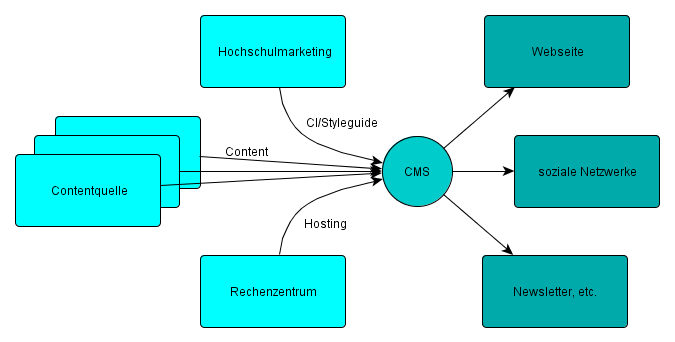
\includegraphics[width=10cm]{kapitel/gruppe3/bilder/verteilter_publishing_workflow}
	\caption{Verteilter Publishing Workflow}
	\label{fig_publishing_workflow}
\end{figure}

Das Hosting wird dabei durch das Rechenzentrum realisiert, während das Hochschulmarketing mit Corporate Identity und Styleguide eine einheitliche Erscheinung der Auftritte leistet. Die Inhalte steuern mehrere, unabhängigen Autoren bei, die mittels unterschiedlicher Berechtigungen und Adressierungen unterschiedliches Publikum erreichen können.
So kann ein unidentifizierter Besucher der Webseite öffentliche, allgemeine Informationen vorfinden, ein angemeldeter Studierender jedoch zusätzlich und prominenter Informationen und Neuigkeiten zu seinem Fachbereich und seinen Kursen.
Weiterhin kann mit einem Content Management System geleistet werden, dass Autoren Inhalte beisteuern und veröffentlichen können, ohne im einzelnen mit den technischen Einzelheiten des Hostings oder des Designs belangt zu werden. Auch können Content Management Systeme Inhalte für weitere Plattformen aufbereiten, zum Beispiel an soziale Netzwerke posten. \footnote{vgl. \cite{content_management_system_patent}}

\subsection{Internes Hochschulmarketing}
\label{subsection_internes_hochschulemarketing}
Im Gegensatz zur Situation in einem Unternehmen genießen einzelne Fachbereiche und Personen in einer Hochschule einen hohen Grad an Freiheit und Autonomie. Daher können in Arbeitsgruppen und Gremien beschlossene Prozesse und Software nicht per Anordnung durchgesetzt werden, sondern müssen nach innen vermarktet werden, um akzeptiert zu werden. Herausfordernd ist hier besonders die Heterogenität, da der technische und fachliche Hintergrund sich unter Mitarbeitern und Fachbereichen erheblich unterscheiden, etwa zwischen technischen und nichttechnischen Fachbereichen.

\subsubsection{Fokussierter Support}
Eine Möglichkeit, Benutzer hin zu einer präferierten Lösung zu leiten ist diese in Präferenzen, Anleitungen und FAQs an erster Stelle und in höherem Detailgrad zu präsentieren. Vielfach wird eine Voreinstellung einfach übernommen, und die erste Lösung zu einer Fragestellung als Referenz angesehen, vergleichbar dem Agenda-Setting.\footnote{vgl. \cite{bonfadelli_medienwirkungsforschung_2015}}

\subsubsection{Schulungen}
Eine weitere Maßnahme ist, Schulungen für die präferierten Lösungen anzubieten, die Vorteile der gefundenen Lösung gegenüber anderen herausstellt. Optimal ist eine solche Lösung transparent, oder aber bietet Alleinstellungsmerkmale, die eine Verwendung aus sich heraus attraktiv erscheinen lassen. Trotzdem kann es vorkommen, dass in Lern- und Umstellungsphasen Lernkurven in der Benutzung absolviert werden müssen. Soll eine Lösung akzeptiert werden, dann muss diese Lernkurve entsprechend begleitet werden.

\subsubsection{Integration}
Eine weitere starke, aber arbeitsintensive Maßnahme ist, die präferierte Lösung stark zu integrieren. Beispielsweise sei die Erstellung von hochwertigen Dokumentvorlagen entsprechend der Corporate Identity für die präferierte Textverarbeitung genannt.

Der Übergang zum fokussierten Support ist hier fließend. Wird die präferierte Lösung an das bestehende System angepasst, so kann von Integration gesprochen werden, wird das System an eine präferierte Lösung angepasst, ist dies fokussierter Support. Beides kann sehr gut gegenseitig ergänzend eingesetzt werden.
\section{Support und Fortentwicklung - AE}
Support und Fortentwicklung hängen hier eng zusammen, da die Fortentwicklung 
hauptsächlich durch die im Support gewonnenen Einsichten über Defizite in Prozessen 
getrieben werden soll. So sollen Diskrepanzen zwischen Erwartungen an das System und 
dessen tatsächlichen Fähigkeiten und Nutzung aufgedeckt und behoben werden.

\subsection{Support}
Supportleistung an einer kleinen Hochschule geschieht häufig direkt und 
unbürokratisch.\footcite{gunter_muller_interview} Dieser ad-hoc-Ansatz bringt 
zwar vielfach schnelle Hilfe, aber nur wenig zuverlässige Informationen über Prozessdefizite.

\subsubsection{Zentrale Dokumentation}
Die Vorteile dieser Art der Hilfeleistung sind für eine kleine Hochschule allerdings evident. 
Der Overhead mehr reglementierter Supportsysteme würde einen unverhältnismäßigen 
Personalaufwand mit sich bringen, und Hilfeleistung verzögern. Die Qualität des 
Supportprozesses selber würde damit sinken.\footcite{gunter_muller_interview}

Notwendig zur besseren Identifizierung von Prozessdefiziten ist allerdings keine 
zentralisierte Supportleistung an sich, sondern lediglich eine zentralisierte Dokumentation 
des geleisteten Supports. Die Abbildung \ref{fig_zentraler_supportlog} verdeutlicht, dass geleisteter Support von 
vollkommen unabhängigen Stellen zentral dokumentiert werden kann.

\begin{figure}[h!]
	\centering
	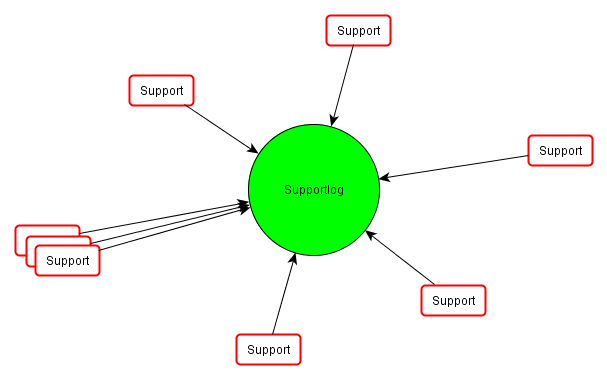
\includegraphics[width=\textwidth]{kapitel/gruppe3/bilder/grafik_supportlog}
	\caption{Unabhängige Supportleister dokumentieren in zentralem Log}
	\label{fig_zentraler_supportlog}
\end{figure}

Es ist dabei unerheblich, ob die Supportleister die Unterstützung als Kern ihrer Aufgabe 
leisten, oder ob es sich um kollegiale Unterstützung bei einem Problem handelt. Gerade 
letztere Information aufzufangen ist wichtig, da diese sonst nur eine sehr schwer 
einzuschätzende Größe bleibt.

Dieser Dokumentationsoverhead ist gering gegenüber dem Overhead eines stark 
reglementierten Supportsystems, erhält alle Vorteile unbürokratischer, schneller 
Hilfeleistung und fängt zusätzlich Informationen über Art und Umfang gelisteten Supports 
auf.

\subsubsection{Knowledge Base}
Aus dem Supportlog kann eine durchsuchbare Knowledge Base aufgebaut werden, die nicht 
nur die allgemeinen Fehlerquellen und Schwierigkeiten von Software im Einsatz beleuchtet, 
sondern ganz speziell die an der Hochschule Emden/Leer in dieser Zusammenstellung 
einmaligen Konfiguration vorliegenden Probleme.

Dadurch kann sehr viel schneller auf spezifische Fehlerszenarien reagiert werden, als dies 
mit allgemeinen Informationen möglich ist, die erst auf die Verhältnisse vor Ort bezogen 
werden müssen.

Auch können aus dem Supportlog FAQs abgeleitet werden, die tatsächlich dem Wortsinn 
nach Listen häufig gestellter Fragen und Antworten darstellen, und nicht was mehr oder 
minder begründet vermutet wird. Eine Diskrepanz mag sich hier durch die Besonderheit von 
Hochschulen ergeben, ein sehr heterogenes Benutzerfeld abzudecken. So mag es 
Nutzergruppen geben, die ein ähnliches Maß an technischer Kompetenz aufweisen wie 
Personal, das ein bestimmtes System betreut, bis hion zu Benutzergruppen, die weit weniger 
oder deutlich andere technische Kompetenz aufweisen.

Auch zeigt sich in den Häufigkeiten bestimmter Probleme, wo spezielle Dokumentation und 
Hilfetexte notwendig sind, die ebenfalls hinterlegt werden können.

Hierzu muss das Supportlog allerdings von einer geeigneten Stelle regelmäßig gesichtet 
werden.

\subsection{Fortentwicklung}
Eine Konzeption kann nur aktuelle Trends und Entwicklungen berücksichtigen. Es ist 
schwierig vorauszuschauen, was die Zukunft danach bringen wird, welche Trends mehr oder 
weniger wichtig sind, und welche Trends darauf folgen werden.

Allerdings ist es keine Frage, dass eine Hochschule länger Bestand hat, und es damit 
sinnvoll ist, Prozesse zu hinterlegen, die neue Trends und Entwicklungen zwar nicht 
vorwegnehmen können, aber deren zeitnahe Entdeckung und Integration ermöglichen.

Auch zeigt sich in der Praxis, dass unvorhergesehene Bedingungen und Ereignisse 
theoretisch gut ausgearbeitete Prozesse und Infrastrukturen übermäßig blockieren können, 
und eine Anpassung geschehen muss. Beispielhaft sei hier für die Hochschule Emden/Leer 
der Trend angeführt, dass Mitarbeiter und Studierende eigene, WLAN-fähige Geräte 
mitbringen und im Netzwerk der Hochschule anzumelden. Das vormals ausreichend 
dimensionierte Netz wurde durch einen Trend unter- oder zumindest 
fehldimensioniert.\footcite{gunter_muller_interview}

\subsubsection{Feedback}
Zur effektiven Begegnung neuer Trends muss an jedem Punkt des Gesamtsystems dem 
Benutzer möglich sein, Feedback zu geben. Mehr noch muss gerade bei neuen oder 
überarbeiteten Prozessen dieses Feedback eingefordert werden, um die Qualität des neuen 
Prozesses oder Tools einschätzen zu können.

Das Feedback gelangt an die zuständige Stelle, muss aber auch zentral gesammelt werden, 
ähnlich wie das Supportlog. Diese Sammlung wird zentral ausgewertet, um verdeckte, 
verteilte Probleme aufzudecken, die sich in Feedback an unterschiedliche Stellen verbergen 
können.

Auf die Auswertung muss, wo sich Probleme zeigen, eine Information der zuständigen Stelle 
folgen, damit eine Verbesserung erarbeitet werden kann. Entsprechend ist die zuständige 
Stelle berechtigt, ein Meeting einzuberufen, damit ihre Eingaben nicht einfach verloren gehen 
können, sondern zwangsläufig mindestens einmal besprochen werden.

\subsubsection{Innovationseingabe}
In den Feedbackprozess eingebettet muss die Möglichkeit für jede Person sein, Innovationen 
aus beliebiger Quelle zu beschreiben, so dass Entwicklungen nicht erst von bestimmter 
Stelle wahrgenommen werden müssen, um erwägt zu werden. Damit kann von beliebiger 
Stelle aus eine Verbesserung in Diskussion gebracht werden.

Damit diese Möglichkeit von Benutzern angenommen wird, muss auf Eingaben angemessen 
schnell reagiert werden. Um eine ernsthafte Reaktion zu gewährleisten, müssen diese 
Vorschläge auch diskutiert worden sein. Daraus ergibt sich ein angemessen kurzer Turnus 
der Auswertung von Support- und Feedbacklog.

\subsubsection{Erfahrungsgetriebene Fortentwicklung}
Aus den Erkenntnissen über Schwachstellen aus dem Supportlog, den Benutzerberichten und 
-bewertungen aus dem Feedbacklog und den Innovationseingaben können nicht nur 
Schwachstellen und Fehler in Prozessen identifiziert werden, sondern auch Trends in der 
Benutzung des Systems erkannt. Da Support und Feedback andauernde Prozesse sind, ergibt 
sich daraus ein selbstregulierendes System, das, wenn die Messgrößen Supportlog und 
Feedbacklog angemessen berücksichtigt werden, evolutionär verbessert wird.

\begin{figure}[h!]
	\centering
	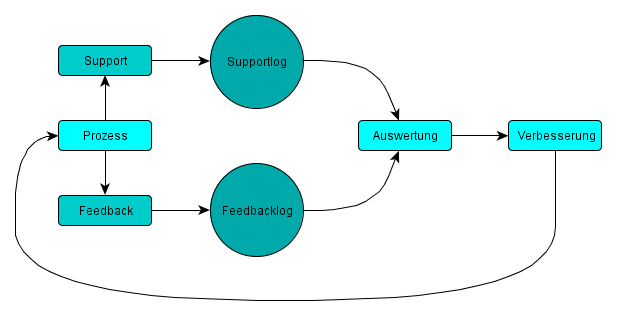
\includegraphics[width=\textwidth]{kapitel/gruppe3/bilder/zyklus_prozessverbesserung}
	\caption{Zyklus der Verbesserung eines Prozesses}
	\label{fig_zyklus_prozessverbesserung}
\end{figure}

Abbildung \ref{fig_zyklus_prozessverbesserung} illustriert den Zyklus folgendermaßen: Ein Prozess existiert und läuft im 
normalen Betrieb. Bei Problemen wird Support geleistet, der im Supportlog vermerkt wird. Zu 
dem Prozess wird zusätzlich Feedback gegeben, das im Feedbacklog festgehalten wird. Beide 
Logs werden ausgewertet und zur Verbesserung des Prozesses herangezogen. Der 
verbesserte Prozess tritt an die Stelle des ursprünglichen Prozesses, der Zyklus beginnt auf 
Basis des verbesserten Prozesses erneut.





















%\section{Hard- und Software - HS}

Das folgende Kapitel bezieht sich auf den Teil des Informationsmanagements, den 
Wollnik und Krzmar als Ebene der Informations- und Kommunikationsinfrastruktur 
bezeichnen (vgl. Kapitel \ref{chapter_grundlagen_INM}) Zur Integration eines hochschulweiten 
Informationsmanagements können bezüglich der Hard- und Software mehrere Ansätze 
gefahren werden.

Zum einen kann eine ganzheitliche integrierte Lösung verwendet werden. Die Universität 
Hamburg hat einen vollständigen Neuanfang bezüglich der Campussoftware gewagt mit 
der integrierten Gesamtlösung „CampusNet“ der Datenlotsen Informationssysteme GmbH. 
Die Entscheidung dazu resultierte aus der Zusammenlegung mehrerer Fachbereiche mit 
sehr unterschiedlichen Teillösungen zu einzelnen Fakultäten. Die verschiedenen Teillösungen 
waren größtenteils inkompatibel oder aufgrund von Eigenentwicklung schwer 
wartbar.\footcite[Vgl.][38]{dini_webportale_2007}

Laut Günter Müller, Leiter des Rechenzentrums der Hochschule Emden/Leer, existieren 
an besagter Hochschule derart verschiedene Teillösungen nicht. Auch würden sich derzeit
Eigenentwicklungen bewusst auf vernachlässigbare Systeme beschränken. 
Software würde grundsätzlich für die gesamte Hochschule 
eingesetzt.\footcite{gunter_muller_interview}

Der Einsatz einer integrierten Gesamtlösung zur Beseitigung von Inkompatibilitäten und 
schwer wartbaren Eigenentwicklungen kann somit keine Argumentationsgrundlage sein.
Des Weiteren reicht die in dieser Ausarbeitung getätigte Analyse des Ist-Zustands und 
der Anforderungen nicht aus, um einen vollständigen Anforderungskatalog zu bilden, 
auf dessen Grundlage eine integrierte Gesamtlösung gefunden werden kann.

Stattdessen wird auf eine flexible Lösung gesetzt, welche den Einsatz einzelner 
Fachanwendungen zur Lösung bestimmter Probleme vorsieht. Personelle und 
finanzielle Ressourcen sind dadurch flexibler einsetzbar, auf veränderte Anforderungen 
an eine Lösung kann flexibler reagiert werden und die Abhängigkeit von einem 
Anbieter für alle Anwendungen wird aufgelöst.

Dies ermöglicht eine schrittweise Migration in Form einzelner Projekte. 
Mögliche Strategien dafür werden in Abschnitt \ref{section_migrationskonzepte} näher erläutert. 

\subsection{Kernanforderungen}
Bei Core-Systemen wird weiterhin auf Appliance Lösungen gesetzt. Das minimiert 
Fehlerpotenzial und den operativen Betrieb. \footcite{gunter_muller_interview}

Softwaresysteme laufen auf virtuellen Maschinen. Die bessere Hardwareauslastung 
und Möglichkeit der automatisierten Administration kann finanzielle und 
personelle Ressourcen sparen.\footcite[Vgl.][198]{baun_servervirtualisierung_2009}
Die Systeme sind somit weniger abhängig von der Hardware, was dessen Austausch 
erleichtert. Netzwerkanbindung, Rechenleistung und Speicherkapazität sind somit 
flexibler an sich verändernde Anforderungen anpassbar.

Die eingesetzte Software soll in die Systemlandschaft integrierbar, lösungsorientiert und 
möglichst barrierefrei sein. Um weiterhin verschiedene Teillösungen und Eigenentwicklungen 
zu vermeiden, sollte bei neu einzuführenden Systemen immer geprüft werden, ob bereits 
eine brauchbare Lösung am Markt exisitert.

Da auch das Übertragungsmedium entscheidend zur Erfüllung 
von Informationsbedarfen ist, wie in Abschnitt \ref{subsection_koordination_informationslogistik} 
näher erläutert wurde, soll der Zugang zu Informationen möglichst unabhängig von 
Client-seitig eingesetzten Systemen sein bzw. Unterstützung für möglichst viele 
Zugriffsarten bieten. Diese Freiheit in der Wahl des Mediums unterstützt den Ansatz der 
Freiheit in Forschung und Lehre.

Eine Client-seitige Systemunabhängigkeit kann durch Webanwendungen im Sinne des 
Ansatzes Software as a Service (SaaS) erreicht werden. Um möglichst alle gängigen Browser 
und Endgeräte zu unterstützen, sollten die Anwendungen den Standards des World Wide 
Web Consortiums (W3C) und, soweit möglich, dem Ansatz responsive design gerecht werden. 
Dadurch kann auch dem Trend bring your own device Rechnung getragen werden, wie in 
Abschnitt \ref{netzinfrastruktur_consumerization_und_byod} näher erläutert wurde.

\subsection{Bereichsübergreifende Basissysteme}
Auch wenn eine Hochschule bestimmte Besonderheiten aufweist - vgl. Abschnitt \ref{anwendung_des_inm_auf_hs} - 
fallen dort informationstechnologische Aufgaben an, für die eine zentrale IT-gestützte 
Lösung geschaffen werden kann. Das verringert redundante Daten und Systeme, sowie 
administrative Aufwände. Im folgenden werden Lösungen für einzelne Aspekte des 
Informationsmanagements aus IT-Sicht vorgestellt, die in allen Aufgabenbereichen von 
Hochschulen genutzt werden können. Weiterhin dienen die Lösungen teilweise als Grundlage 
für spezialisierte Systeme oder ermöglichen hilfreiche Erweiterungen dieser.

\subsubsection{Identity Management}
Um die Anzahl an verschiedenen Accounts zu minimieren, sollten die Benutzer zentral gepflegt werden. 
Dies kann in einem Verzeichnisdienst, wie dem bereits eingeführten Active Directory\footcite{gunter_muller_interview}
geschehen. Die Authentifizierung für ein System findet dann nicht am jeweiligen System selbst statt, sondern 
geschieht mit Hilfe des Verzeichnisdienstes. Vorteil ist, dass die Benutzenden sich nur einen Anmeldenamen 
zzgl. Kennwort merken müssen, um sich an den verschiedenen Systemen anzumelden. Weiterhin gilt eine 
Aktualisierung von Informationen global, wodurch Inkonsistenzen aufgelöst werden.

Davon ausgenommen dürfen Systeme sein, deren spezielle Sicherheitsanforderungen nicht mit diesem Konzept 
vereinbar wären. Auch muss die Authentifizierung gesichert geschehen und eine regelmäßige Kennwortänderung 
forciert werden. Auf bestehende Sicherheitsaspekte wurde in Abschnitt \ref{subsection_sicherheitsaspekte} bereits 
eingegangen.

Zuzüglich zum zentralen Verzeichnisdienst ist auch ein SingleSignOn Mechanismus 
empfehlenswert\footnote{siehe Abschnitt \ref{subsubsection_identitatsmanagement}}, 
wie es an der Universität Augsburg durch das System Webauth umgesetzt ist.\footcite[Vgl.][206]{digicampus_2009}

Die an der Hochschule Emden/Leer eingesetzten Websysteme sollen, soweit möglich, vollständig auf SSO umgestellt werden, um dem Benutzer eine möglichst integrierte Landschaft zu bieten. Dies gilt dann auch für einzuführende Systeme. Weiterhin sollte jedes System aus Sicherheitsgründen insofern angepasst werden, dass auch ein SingleSignOff möglich ist.\footcite[Vgl.][150]{kloetgen_2012} Diese zentrale Abmeldung soll gewährleisten, dass die Benutzenden auf allen Systemen, auf denen sie sich bewegt haben, mit einem Klick abgemeldet sind. Der Diebstahl von Websessions bzw. die Fremdnutzung durch Benutzer, die einen Computer anschließend nutzen, kann damit vermieden werden.

Die meisten Systeme bieten eine Benutzerdatenpflege durch den Benutzer selbst an. Diese muss auf den einzelnen Systemen ausgeschaltet sein. Die Benutzenden sollten dennoch die Möglichkeit haben ihre Daten eigenständig zu ändern, allerdings ausschließlich über ein zentrales Formular. So wird ein konsistenter Datenbestand gesichert. Insofern die Informationen in anderen Systemen benötigt werden, müssen diese vom zentralen System wiederkehrend angefordert oder, wenn die Daten im System persistiert sein müssen, automatisiert und über gesicherte Verbindungen verteilt werden.

Ein weiterer Vorteil zentraler Benutzerdaten ist, dass diese zentral ausgewertet werden können. Informationen über Personen können mit Informationen anderer Art aus anderen Systemen angereicht werden um diese weiterzuverwenden. So können automatisierte Reports über Forschungsprojekte erstellt werden, Expertisen zu bestimmten Themen identifiziert werden oder Verknüpfungen von Personen zu verwaltungstechnischen Aufgaben bereitgestellt werden, wie zum Beispiel die Exmatrikulation. Die Umsetzung ist dabei individuell an die Gegebenheiten und Informationsbedarfe der Hochschule anzupassen. Aus diesem Grund wird die technische Lösung eine Individuallösung werden. Diese Individuallösung sollte ein Teil Campus Portals werden, auf das in Abschnitt \ref{subsubsection_campus_portal} eingegangen wird. 

\subsubsection{Geschäftsprozesse}
+Trotz der Freiheit in Forschung und Lehre gibt es an Hochschulen Geschäftsprozesse, die in der Regel immer gleich ablaufen. Bei verstärkter Prozessorientierung werden außerdem vermehrt solche Prozesse entstehen. Ein häufiges Problem bei Geschäftsprozessen ist, dass Personen unterschiedlichster Bereiche involviert sind und die Prozesse häufig nicht transparent genug sind.\footcite[Vgl.][12]{becker_prozesse_2010}

Hier empfiehlt sich der Einsatz von Business Process Management (BPM). BPM dient der Identifizierung, Dokumentation und Verbesserung von Prozessen. Die allgemeine Herangehensweise ist dabei folgende. Nach dem Identifizieren möglicher Prozesse werden diese modelliert, konkretisiert und digitalisiert. Tool unterstützen beim Durchlaufen der digitalisierten Prozesse. Der Verbesserungsprozess, sprich die Anpassung der Prozesse, findet kontinuierlich statt.

Die Modellierung der Prozesse im ersten Schritt sollte auf abstraktem Niveau stattfinden. Dies erleichtert den Einstieg und macht Verbesserungspotenziale sichtbarer. In der WWU Münster wurde dafür die PICTURE Methode verwendet.\footcite[Vgl.][16]{becker_prozesse_2010} Wichtig ist die Einbeziehung der Prozessbeteiligten. Abschnitt \ref{section_changemanagement} setzt sich mit den Besonderheiten des Change Managements an Hochschulen detaillierter auseinander.

Im zweiten Schritt kann der ggf. angepasste Prozess konkretisiert und in Form des Industriestandards Business Process Model Notation (BPMN) digital notiert werden. Ein Client-Tool zur Erstellung von BPMN ist das Activiti BPMN 2.0 Eclipse Plugin.\footcite{eclipse_bpmn2_modeler}

Mit Hilfe der zentralen Business Process Management (BPM) Platform activiti können die Prozesse aktiv den Workflow verbessern, Konsistenz wahren und zeitliche Ressourcen sparen.  Die Plattform ermöglicht REST Anfragen, wodurch die Prozessinformationen auch in andere Applikation integriert werden können. Der Activiti Explorer ermöglicht den voll funktionalen Zugriff via Weboberfläche. Somit wird der Kernanforderung SaaS Rechnung getragen. Weiterhin ist Activiti Open Source und somit ausbau- und anpassungsfähig.\footcite{activiti_website}

Durch activiti wird es möglich sein die Automatisierung von einzelnen Prozessen Stück für Stück voranzutreiben indem manuelle Aufgaben gegen Automatismen ersetzt werden. Einzelne Teile des Workflows können dann automatisiert Scripte starten, E-Mails verschicken und ähnliches und somit stückweise die manuelle Bearbeitung reduzieren. Durch Definition von Pflichtfeldern für einzelne Prozessschritte können vorab benötigte Informationen festgelegt werden, sodass Nachfragen vermieden werden.

\subsubsection{Content Management}
Um den wachsenden Anforderungen in Bezug auf Content Management genüge zu tun, wurde an der WWU Münster das Enterprise Content Management System Alfresco eingeführt. Auch an einer kleinen Hochschule kann ein solches System eingesetzt werden. Alfresco bietet diverse Vorteile. Die für dieses Konzept Relevanten werden hier kurz aufgelistet:\footcite[Vgl.][47 ff.]{kloetgen_2012}

\begin{itemize}
	\item Unterstützung für mobile Endgeräte
	\item Anpassungs- und ausbaufähig
	\item diverse Zugriffsmöglichkeiten zur Nutzung innerhalb bekannter Standardanwendungen
	\item Publikation in sozialen Netzwerken
	\item Unterstützung verschiedener Standardschnittstellen
	\item Activiti Workflow Engine
	\item Metadaten
\end{itemize}

Alfresco bietet damit die ideale Grundlage verschiedenste Informationen zu verwalten, sowie die Unterstützung des vollständigen Dokumenten-Lifecycles: von der Erstellung über die Bereitstellung bis zur Archivierung.

Die Art des Zugriffs auf Dokumente ist dynamisch dank der Unterstützung zahlreicher Standards. Somit kann eine Integration des Zugriffs auf Dokumente, angepasst an die jeweiligen Anforderungen eines benutzenden Systems, geschehen. Ein Dokument, welches an verschiedenen Orten auf verschiedene Arten bereitgestellt werden soll, kann dank Alfresco zentral aktualisiert werden. Die zugreifenden Systeme erhalten immer genau den Lifecyle-Version des Dokuments, der für sie vorgesehen ist.

Dank der integrierten Versionierung entfällt außerdem der aufwendige Wiederherstellungsprozess bei Dateisystem-basierten Sicherungen.

Durch die Möglichkeit Metadaten anzugeben, wird der Weg für eine brauchbare Dokumentensuche geebnet. 
Diese kann in die integrierte Gesamtsuche einbezogen werden.\footnote{siehe Abschnitt \ref{subsubsection_integrierte_gesamtsuche}}

\subsection{Spezialsysteme}
Unter Spezialsystemen sind hier Softwarelösungen zu verstehen, die bei speziellen Aufgaben im Hochschulalltag unterstützen sollen, wie zum Beispiel die Bereitstellung von Lehrmaterial oder die Evaluation von Kursen.

\subsubsection{Lernplattform}
Die Hochschule Emden/Leer setzt bereits erfolgreich und in allen Fachbereichen das System moodle als Lernplatform ein.\footcite{gunter_muller_interview} 
Die Nutzung der Funktionen variiert dabei jedoch zwischen den einzelnen Fachbereichen.\footnote{siehe Abschnitt \ref{subsection_e-learning}}
Solange moodle die Anforderungen der Hochschule an eine Lernplattform erfüllt, besteht kein Grund das System auszutauschen.

Neben den bereits genutzten Standardfunktionen ist moodle ausbaufähig.

Beim Aufruf von moodle soll die Authentifizierung durch einen SSO Mechanismus geschehen. Für das Lernraumsystem moodle gibt es bereits ein SSO Plugin.\footcite{macklin_moodle_sso_plugin} Integriert werden sollte, wie in Kapitel 6.3.2.1 erläutert, dann auch ein Single-Sign-Off Mechanismus.

Statt der Stammdatenänderung via moodle wird der entsprechende Menüpunkt ausgeblendet werden bzw. die Benutzenden auf ein zentrales Formular weiterleiten, um persönliche Informationen zentral und damit konsistent zu halten.

Die in den Kursen zur Verfügung gestellten Dateien jeglicher Art werden in Alfresco gepflegt und von moodle angebunden. Die entsprechenden Schnittstellen und Plugins existieren bereits auf dem Markt und müssen somit nicht neu entwickelt werden.

Vorteil der Integration von Alfresco in moodle ist, dass damit die Vorteile Alfrescos zur Dokumentenverwaltung genutzt werden können. In moodle kann dann eine bestimmte Version oder die jeweils aktuellste referenziert werden. Bei den Dokumenten kann es sich um Textdokumente, Audio- oder auch Videodateien handeln. Durch Alfrescos Unterstützung für mobile Endgeräte wird den Zugreifenden die Möglichkeit gegeben, ein Dokument auf verschiedensten Endgeräten anzuzeigen bzw. wiederzugeben. Außerdem können dank Alfresco diese Dokumente nicht nur innerhalb von moodle via Weboberfläche aufgerufen werden, sondern über verschiedene Medien angebunden werden, zum Beispiel via Filesystem in Form eines Netzwerk-Shares. 
Damit wird eine Freiheit in der Wahl des Übertragungsmedium gewährleistet.\footnote{siehe Abschnitt\ref{subsection_koordination_informationslogistik}}

Ein mögliches Migrationskonzept wird in Abschnitt \ref{subsubsection_changemanagement_alfresco} erläutert.

\subsubsection{Publikationen}
Um Wissenschaftler bei der Publikation von Zeitschriften zu unterstützen, kann die Plattform Open Journal System (OJS) eingesetzt werden, wie es auch in der WWU Münster getan wird. Es bietet die Möglichkeit elektronische Zeitschriften zu verwalten und den gesamten Publikationsworkflow abzubilden.\footcite[Vgl.][48]{vogl_fortschritte_2012}

Zusätzlich sollte auch ein Workflow in activiti implementiert werden, der bei der Publikation unterstützt. So können wichtige Metadaten aufgenommen und an relevante Systeme weitergegeben werden. Ändern sich Systeme oder kommen neue hinzu, müssen sich Wissenschaftler nicht umgewöhnen, sondern nutzen weiterhin den in activiti hinterlegten, für die neuen Systeme jedoch angepassten, Prozess. Dadurch besteht auch die Möglichkeit ein publiziertes Dokument zusätzlich in Alfresco abzulegen, wenn ein Anwendungsfall dies benötigt.

OJS bietet die Möglichkeit der Authentifizierung via Single Sign On. Dies geschieht via Shibboleth.\footcite{ojs_setup_sso} 
Neben der Konfiguration von SSO sollte auch hier wieder den Benutzenden die Möglichkeit des Single-Sign-Offs gegeben werden.

\subsubsection{Evaluation}
Wie auch die Universität Münster\footcite{evasys_muenster} und die TU Dortmund\footcite{evasys_dortmund} setzt die Hochschule Emden/Leer bereits die Software EvaSys zu Evaluationszwecken ein.\footcite{gunter_muller_interview} Sie ist webbasiert und entspricht damit dem SaaS Prinzip.
Seit Version 5 unterstützt EvaSys auch die SSO Authentifizierung\footcite{evasys_sso}, welche auch an der Hochschule Emden/Leer eingesetzt werden soll.

\subsubsection{Campus Portal}
\label{subsubsection_campus_portal}
Ein Campus Portal dient als zentrale Anlaufstelle für alle Hochschulangehörigen und ist ein personalisiertes Webportal. Es soll die Verwaltung persönlicher Daten ermöglichen, eine Übersicht über informationstechnische Funktionen, inklusive Weiterleitung zum entsprechenden System, integrieren, sowie aktuell relevante personalisierte Informationen in Form einer Agenda anzeigen. Das Campus Portal dient also als Startpunkt.

Hinter den informationstechnischen Funktionen stecken alle Werkzeuge und Spezialsysteme, die einem bestimmten Zweck dienen. Auf einige davon wurde in den vorhergehenden Unterkapiteln bereits eingegangen. Bei der Integration solcher Systeme werden nun die anfangs genannten Kernanforderungen an solche Systeme, nämlich integrierbar und systemunabhängig (SaaS) zu sein, deutlich.

Ein solches Campus Portal ist vor allem der Informationsübersicht dienlich. Durch personalisierte und dynamisch generierte Inhalte gewinnen die Benutzenden einen Überblick über die Informationen\footcite[Vgl.][24]{dini_webportale_2007}, die sonst ausschließlich in den verschiedenen Systemen verteilt sind. Der Aufbau eines Campus Portals und die Integration der Spezialsysteme kann schrittweise erfolgen, sollte jedoch zur Akzeptanzgewinnung bei Veröffentlichung eine gewisse Menge externer Systeme integrieren.\footcite[Vgl.][17 f.]{dini_webportale_2007} Die Universität Karlsruhe hat im ersten Schritt das Veranstaltungsmanagement und die Prüfungsverwaltung der Software-Systeme der HIS GmbH in das Portal integriert.\footcite[Vgl.][40 f.]{dini_webportale_2007}

Aufgrund der Individualität der fachlichen und technischen Anforderungen wird es an der Hochschule Emden/Leer wahrscheinlich auf eine Individuallösung hinauslaufen.\footcite[Vgl.][21]{dini_webportale_2007} Vorsicht! Die Aufwände für die Umsetzung eines Campus Portals sind in der Kosten- und Zeitschätzung für das Redesign der Hochschul-Webseite nicht integriert.

Orientiert am Anforderungskatalog der WWU Münster an ein solches Portal und unter der Voraussetzung, dass die in diesem Konzept genannten Systeme 
umgesetzt werden, kann ein zukünftiges CampusPortal der Hochschule Emden/Leer folgende Informationen konsolidieren:\footcite[Vgl.][158 ff.]{vogl_fortschritte_2012}

\begin{itemize}
	\item Kalender
	\begin{itemize}
		\item Abonnement-Prinzip
		\item inklusive Detailinformationen, zum Beispiel Kontoinformationen für Rückmeldegebühren
		\item Agenda aus moodle
	\end{itemize}
	\item Referenz zu gewählten Kursen (moodle)
	\item Referenz zum E-Mail-Portal (Outlook Web App)
	\item Suchmaschine
	\item offene Tasks im BPM System
	\item Start möglicher Tasks im BPM System (zum Beispiel Workflow für die Publikation)
	\item offene Evaluationen
\end{itemize}

Neben den in diesem Konzept genannten Systemen, könnten weitere Spezialsysteme in das Campus Portal integriert werden, sofern diese entsprechende Schnittstellen aufweisen. Der Anforderungskatalog der WWU Münster enthält außerdem:

\begin{itemize}
	\item Stundenplan
	\item Vorlesungsverzeichnis inkl. Details
	\item Leistungsübersicht
	\item Hochschulleben
	\begin{itemize}
		\item Mensapläne
		\item Hochschulsport
		\item Veranstaltungen
	\end{itemize}
	\item Einführung in die Benutzung
\end{itemize}

Alternativ zur Einführung in die Benutzung kann auch das Konzept eines Hilfesystems integriert werden, das via Sprechblasen Hilfestellungen oder Erläuterungen anzeigt zur jener Funktionalität, auf der sich der Mauszeiger gerade befindet.\footcite[Vgl.][22]{vogl_bericht_2013}

Die technische Struktur kann analog zu der des Portals myWWU der Universität Münster aufgebaut sein, wie im Folgenden abgebildet.\footcite[Vgl.][165]{vogl_fortschritte_2012}
\begin{figure}[h!]
	\centering
	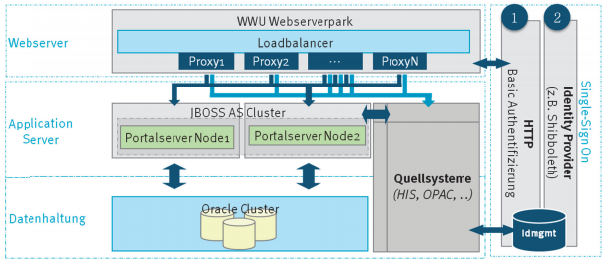
\includegraphics[width=\textwidth]{kapitel/gruppe3/bilder/struktur_mywwu}
	\caption{technische Struktur des Portals myWWU der Universität Münster}
	\label{fig_struktur_mywwu}
\end{figure}
\newpage

\subsubsection{Integrierte Gesamtsuche}
\label{subsubsection_integrierte_gesamtsuche}
Wissenschaftliche Informationen sind häufig in verschiedenen Systemen angesiedelt. Durch die Einführung eines Systems zur integrierten Gesamtsuche würde die Suche an zentraler Stelle ausgeführt. Einzelne Systeme werden von den Suchenden nicht vergessen und die Integration neuer wissenschaftlicher Informationssysteme wird dauerhaft kommuniziert statt einmalig, wie es beispielsweise beim 
Versand einer Info-E-Mail der Fall wäre.

Die WWU Münster nutzt dafür einen „Suchmaschinen-basierte[n] Ansatz auf Basis der Software Primo von der Firma Ex Libris“.\footcite[Vgl.][41]{vogl_fortschritte_2012} Dafür nötig ist eine Normalisierung der Datenformate interner und externer Quellen, welche „insbesondere auf der Detailebene […] aufwändige Anpassungen und Eigenentwicklungen notwendig“ machen.\footcite[Vgl.][42]{vogl_fortschritte_2012}

Quellsysteme, ausgehend von diesem Konzept, können sein:
\begin{itemize}
	\item Alfresco
	\item Identity Management System
	\item ForschungsDB Niedersachsen
	\item moodle
	\item Open Journal System
	\item Hochschulexterne Informationssysteme wie zum Beispiel video2brain
	\item ggf. Bibliothekssuche
\end{itemize}

Wichtig ist neben korrekten und vollständigen Ergebnissen auch die Benutzbarkeit. Bekannte Funktionalitäten aus anderen Suchmaschinen, wie Gruppierungen, sollten integriert sein, wie auch eine übersichtliche und funktionale Benutzeroberfläche.\footcite[Vgl.][43]{vogl_fortschritte_2012}

\subsection{Ausblick bei Integration der Bibliothek}
Auch wenn die Bibliothek in dieser Ausarbeitung ausgenommen ist, muss erwähnt werden, dass bei Informationsmanagement-Projekten anderer Hochschulen und Universitäten auch die Bibliotheken integriert werden. Die über die Bibliothek zur Verfügung gestellten Informationen werden vor allem für Forschung und Lehre genutzt, welches die Kernaufgaben von Hochschulen sind.

Dementsprechend kann die Integration der Bibliothekssuche in die integrierte Gesamtsuche zur Aufwertung der Suchergebnissen beitragen. Um auch nicht digital verfügbare bzw. archivierte Zeitschriften und Bücher integrieren zu können, kann ein Digitalisierungssystem eingeführt werden. Die WWU Münster setzt dafür vor Ort frei verfügbare Scanner zuzüglich der Software scantoweb ein.\footcite[Vgl.][50]{vogl_fortschritte_2012}

\section{Abwägung des Einsatzes eines Informationsmanagers an der Hochschule Emden/Leer - JL}
\label{section_einsatz_cio}
\textit{Autor: Julia Lübke}

Das Soll-Konzept analysiert die Ist-Situation um den derweilen Zustand der  Hochschule Emden/Leer zu ermitteln. Daraus lässt sich erkennen, ob es generell einer Verbesserung des Informationsmanagements in der Zukunft bedarf und wo diese anzusetzen sind oder ob noch kein Informationsmanagement besteht und aufgebaut werden muss. Dazu sind verschiedene Aspekte zu beleuchten. Neben der Anforderung des zukünftigen Marketings, den technischen Neuerungen und der darauf folgenden Umsetzung ist zu klären, ob die Hochschule Emden/Leer eine Führung im Bereich des strategischen und operativen Informationsmanagements benötigt.

Im klassischen Informationsmanagement ist dies die Aufgabe eines Informationsmanager, dem sogenannten Chief Information Officer. Wie auf der Abbildung \ref{fig_def_inm} zu erkennen, arbeitet der Informationsmanager dabei als zentrale Schnittstelle zwischen technischen, organisatorischen und wirtschaftlichen Teilbereichen und dient dort als sogenannter Mittler zwischen den verschiedenen Bereichen und untersucht dabei die Informations- und Kommunikationstechniken in allen unterschiedlichen Bereichen um diese sinnvoll einzusetzen. 
\footcite[86]{definition_informationsmanager}

\begin{figure}[h!]
	\centering
	\includegraphics[width=10cm]{kapitel/gruppe3/bilder/definition_informationsmanager}
	\caption{Definition Informationsmanager}
	\label{fig_def_inm}
\end{figure}

\subsection{Analyse des Ist-Zustandes}
\label{subsection_analyse_ist_zustand}

Bezug nehmend auf das Organigramm aus Abbildung \ref{fig_organigramm_HS} der Hochschule Emden/Leer und der Bewertung aus  \ref{bewertung_gewichtung} ist festzuhalten, dass der Hochschule kein klassisches Informationsmanagement zugrunde liegt, sondern ein zentrales Informationssystem. Es werden bereits Informationen verwaltet und weitergegeben, jedoch nicht an zentraler Stelle. Zentrale Systeme, siehe Abbildung \ref{fig_zentrale_systeme}, Kapitel \ref{section_zustaendigkeiten}, sowie unterschiedliche Möglichkeiten werden für alle zur Verfügung gestellt und in Anspruch genommen. 

Es gibt keine Verwaltung, sondern verschiedene Bereiche, die unterteilt sind in Arbeitsgruppen, Abteilungen sowie Rechenstelle und Pressestelle. Weiterhin beinhaltet das Informationssystem verschiedene Prozesse zum Datenaustausch bzw. Datenfluss und Back-up-Transfer aus verschiedenen Systemen.  Die Nutzung des gegenwärtigen Informationssystems wird unterschiedlich stark genutzt oder ausgelastet. 

Von den zentralen Einrichtungen nehmen das Hochschulrechenzentrum und die Bibliothek einen wichtigen Platz in der Hochschule Emden/Leer ein. Das Hochschulrechenzentrum übernimmt derweil viele Aufgaben der Informationsverwaltung und Planung. Doch nicht nur da werden Informationen gesammelt und ausgewertet. Die Hochschule in Emden definiert eine ganze Reihe von Arbeitsgruppen, beispielsweise die Arbeitsgruppe Zahlen, Daten, Fakten, die Kennzahlen der Hochschule und der einzelnen Fachbereiche sammelt und diese auswertet und an gewünschte Stellen weitergibt.  

Aktuell besteht keine erweiterte Vernetzung unterschiedlicher Intranetzsysteme zwischen verschiedenen Hochschulen. Lediglich im Bereich der Bibliothek werden Inhalte an mehreren Standorten gemeinsam genutzt. Abschließend ist zu erwähnen, dass die Hochschule Emden/Leer auch keine Einzelperson oder ein Gremium als zentrale Informationsverwaltung nutzt.


\subsection{Betrachtung des zu erwartenden Soll-Zustandes }
\label{subsection_betrachtung_soll}

Nach Betrachtung der Best-Practice-Beispiele aus Kapitel \ref{chapter_best_practice_beispiele} lässt sich erkennen, dass jede Hochschule und auch Universität den Umgang des Informationsmanagements anders angeht. So spielen verschiedene Faktoren eine Rolle, die an jeder Hochschule/Universität unterschiedlich ausgelegt sind. Ein Vergleich der betrachteten Universitäten mit der Hochschule Emden/Leer zeigt, dass Emden eine wesentlich kleinere Institution ist und somit andere Ansprüche hat und weniger komplexe Strukturen besitzt, als beispielsweise die WWU Münster, die über 40.000 Studierende pflegt. 

Trotz unterschiedlich integrierter Möglichkeiten der unterschiedlichen Universitäten zur Umsetzung des jeweiligen Informationsmanagements, gibt es doch Bereiche, die gleich oder zumindest ähnlich sind. So sind Bibliotheken, Gremien, Ausschüsse, ebenso wie Fachbereiche, das Rechenzentrum und auch das Präsidium Teil einer jeden Hochschule oder Universität. 

Es ist also zu schauen, wo sich das Informationsmanagement als zentrale Informationsquelle ansetzen lässt, um mehrere Bereiche und Bestandteile untereinander zu verbinden. Fakt ist, dass es in Emden bereits drei Arbeitsgruppen gibt, die bestimmte Informationen gewinnen und filtern.  So wäre zu betrachten, wie die Zentralisierung einer übergeordneten Informationsquelle und -weitergabe zu bewerkstelligen wäre und wie der Aufbau einer neuen Struktur die Möglichkeit zur Verbesserung des Informationsaustausches aussehen könnte. 

In Kapitel \ref{subsection_zentralisierung_integration} wird beschrieben, dass die meisten Hochschulen und Universitäten unter einer neu geschaffenen Organisation arbeiten. Dabei spielen das Rechenzentrum, die Bibliothek und die Verwaltung immer eine Rolle in einer solchen Organisation. Kein Konzept ist maßgeschneidert und nicht auf jede Hochschule oder Universität anwendbar.

\subsubsection{Empfehlungen der ZKI bezüglich des Informationsmanagers}
\label{subsubsection_zki}

Neben den verschiedenen Projekten und Einrichtungen, die im Kapitel \ref{chapter_best_practice_beispiele} beleuchtet werden, und aufzeigen, wie mit dem Informationsmanagement umgegangen wird, gibt es noch die Zentren für Kommunikation und Informationsverarbeitung (ZKI) in Lehre und Forschung, die Empfehlungen für Hochschulen bezüglich des Informationsmanagements und besonders Empfehlungen für den Informationsmanager aussprechen.

Blickend auf die Publikation der ZKI basierend auf einer Studie der CIOs und IT-Governance an deutschen Hochschulen aus dem Jahre 2014 wurden über mehrere Jahre von der Kommission für IT-Infrastruktur der Deutschen Forschungsgemeinschaft (KfR) hinweg folgende Empfehlungen für Hochschulen ausgesprochen.

Zwischen 2001 - 2005 gab die KfR folgende Empfehlung:

\textit{" Aufgrund der Relevanz der Informationsverarbeitung für alle Bereiche der  Hochschule wird empfohlen, 
	einen Generalverantwortlichen für Information und  Kommunikation (CIO, Chief Information Officer) 
	in der Hochschulleitung oder ein geeignetes Leitungsgremium mit entsprechenden 
	Entscheidungskompetenzen mit der Entwicklung und  Koordinierung aller IuK-Aufgaben 
	zu betrauen."}\footcite[3]{zki_studie_cio_2014}

Zwischen 2006 - 2010 werden weitere Ausführungen genannt:

\textit{" Integriertes Informationsmanagement ist daher zur wesentlichen Aufgabe bei der Planung des 
	Einsatzes moderner Techniken von Information und Kommunikation für die Hochschulen geworden. 
	Eine solche Planung setzt die Position eines Verantwortlichen für Information und Kommunikation 
	als Mitglied der Hochschulleitung (CIO: Chief Information Officer) voraus, wie er in der Wirtschaft 
	und an verschiedenen Hochschulen bereits etabliert ist."}\footcite[16]{zki_studie_cio_2014}

Die KfR Empfehlungen zwischen 2011-2015 werden noch weiter ausgebaut:

\textit{"In der Hochschulpraxis lassen sich vier unterschiedliche Umsetzungstypen beobachten:  Strategischer CIO mit Leitungsfunktion: Ein Vizepräsident - oder eine Vizepräsidentin - ist explizit für das Informationsmanagement zuständig. Teilweise übernimmt auch der Kanzler die Zuständigkeit für das Informationsmanagement.}

\begin{itemize}
	\item \textit{Strategischer CIO mit Stabsfunktion: Ein Hochschullehrer oder IT-Manager - 
		bzw. Hochschullehrerin/IT-Managerin - im Präsidialstab koordiniert das Informationsmanagement.} 
	\item \textit{Operativer CIO: Der Leiter - bzw. die Leiterin - einer zentralen 
		Informationsinfrastruktureinrichtung fungiert gleichzeitig als CIO der Hochschule.}
	\item \textit{Kollektiver CIO: Die CIO-Funktion wird von einem Lenkungsausschuss mit zwei bis 
		drei Personen ausgeübt, der allerdings - anders als die traditionelle Senatskommission - über 
		unmittelbare Entscheidungsbefugnisse verfügt.}
\end{itemize}
\textit{Jede dieser CIO-Umsetzungsvarianten hat ihre Vor- und Nachteile. Es hängt von den 
	Gegebenheiten an den Hochschulen und insbesondere auch von Personen ab, welche 
	Umsetzung die am besten geeignete ist. Wichtig ist, dass der CIO - in welcher Form 
	auch immer - einen unmittelbaren Zugang zur Hochschulleitung hat und die IT-Belange 
	der gesamten Hochschule strategisch - mit unmittelbarer Richtlinien- und 
	Entscheidungskompetenz - fährt und verantwortet."} \footcite[17]{zki_studie_cio_2014}

Abschließend ist zu sagen, dass die ZKI/KfR einer Hochschule eine zentrale Informationsschnittstelle in Form eines CIOs oder eines CIO-Gremiums empfiehlt.

\subsubsection{Informationsmanager oder Gremium als zentrale Informationsschnittstelle}
\label{subsubsection_cio_gremium}

Der Aufbau eines Informationsmanagements bedarf vieler Schritte und Überlegungen (siehe Abschnitt \ref{begriffsdefinition_inm}). Neben den Veränderungen und deren Umsetzung ist zu klären, ob der bisherige Austausch der Informationen der Hochschule Emden/Leer durch eine zentrale Einrichtung oder einer Einzelperson und entsprechenden Verantwortlichkeiten geregelt werden soll. Um dies in ein reales Szenario zu bekommen, sind die Möglichkeiten aufzuzeigen und ein entsprechend passendes Modell für die Hochschule Emden/Leer zu entwickeln. Dazu werden in Kapitel  \ref{chapter_best_practice_beispiele}, ebenso wie in der Studie der ZKI verschiedene Konzepte des Chief Information Officers (CIO) aufgezeigt. 

Ein einheitliches Konzept ist nicht gegeben, sodass nicht jede Lösung auch passend für die Hochschule Emden/Leer ist. Die betrachteten Universitäten haben ein anderes Anforderungsprofil an ein Informationsmanagement und deren zentrale Leitung als Emden, die wesentlich kleinere und weniger komplexe Strukturen besitzt. Zu den betrachteten Best-Practice-Beispielen lassen sich zusätzlich die Empfehlungen der KfR heranziehen. 

Alle haben gemeinsam, dass das Verwalten der Informationen aus einer Schnittstelle heraus geschieht. Auch dieses Konzept ist für die Hochschule Emden/Leer zu überlegen. Nun stellt sich die Frage, wo diese Schnittstelle anzusetzen ist und wer die Aufgaben übernehmen soll. Verschiedene Möglichkeiten sind hier zu betrachten. Zum einen gibt es das Personenmodell, den CIO, beschrieben in \ref{anforderungsprofil_informationsmanager} und \ref{eingliederung_informationsmanager} der die Schnittstelle bildet, zum anderen gibt es die Möglichkeit eines CIO-Gremiums. 


\textbf{Personenmodell:\newline}
Eine Person wird als Informationsmanager herangezogen und übernimmt die in den Abschnitten \ref{aufgaben_funktionen_informationsmanager},\ref{anforderungsprofil_informationsmanager} und \ref{eingliederung_informationsmanager} angegebenen Aufgaben, die hochschulangepasst sind. Dabei ist zu betrachten, wer diese Aufgabe übernehmen soll. Der CIO kann aus der Privatwirtschaft geordert werden. Dabei ist zu bedenken, dass dafür eine Menge Ressourcen benötigt werden. Neben dem aufwendigen Bewerbungsprozess und der Einstellung erfolgt die Einarbeitungszeit und die Einführung des Informationsmanagements durch den CIO. Als weiterer Punkt sind noch die erhöhten Personalkosten in dieser Zeit zu nennen.

Neben der Möglichkeit einen CIO aus der Privatwirtschaft zu holen, besteht auch die Möglichkeit einen hochschulinternen Mitarbeiter zu involvieren. Der Bewerbungszeitraum und die Einarbeitung verringern sich, da ein bestehender Mitarbeiter die Hierarchie und die Arbeitsweise der Hochschule Emden/Leer bereits versteht und kennt. Allerdings ist nicht zu verachten, dass diese Person, entweder eine Mehrbelastung durch die zusätzlichen Aufgaben des Informationsmanagers tragen muss oder für die vorherige Stelle ein neuer Mitarbeiter gesucht werden müsste, was auch in diesem Fall mit einem erhöhten Kosten- und Zeitaufwand verbunden wäre.


\textbf{Gremiummodell:\newline }
Soll das Informationsmanagement allerdings nicht nur von einer einzelnen Person betrieben werden, ist zu klären, wer diese Aufgabe übernehmen soll. Dazu ist immer in Vergleich zu setzen, welche Parameter greifen. Die Studie der ZKI besagt, Bezug nehmend auf die Abbildung \ref{fig_herkunft_cio_hochschulen}, dass die Gremienmitglieder aus ganz unterschiedlichen Bereichen der Hochschule kommen. Ist dies der Fall und ein Gremium wird ernannt, ist ein Arbeitsaufwand der anfallenden CIO Tätigkeiten auf alle Mitglieder aufgeteilt. So ist der Gesamtaufwand pro Person prozentual geringer als bei einer einzelnen Person, die mindestens 50\% ihrer Zeit in CIO-Aufgaben investiert. 



\begin{figure}[h!]
	\centering
	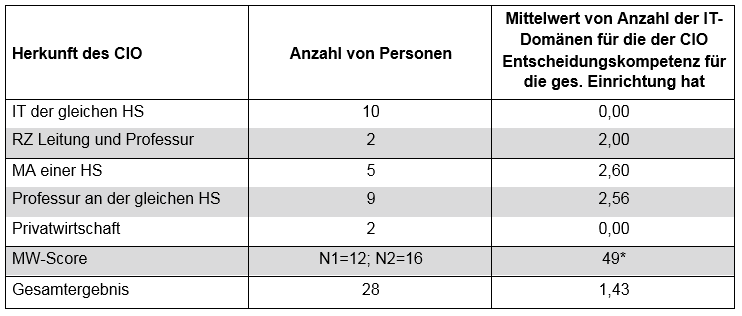
\includegraphics[width=\textwidth]
	{kapitel/gruppe3/bilder/herkunft_cio_hochschulen}
	\caption{Herkunft des CIO an verschiedenen Hochschulen, nach ZKI CIO-Studie}
	\label{fig_herkunft_cio_hochschulen}\footnote{\cite[8]{zki_studie_cio_2014}}
\end{figure}



\subsection{Empfehlung für die Hochschule Emden/Leer}
\label{empfehlung_cio}

Durch stetig wachsende Anforderungen besonders im Bereich der technischen Neuerungen und deren Umsetzung sowie Weitergabe und Verarbeitung von Informationen spricht die KfR seit Jahren Empfehlungen bezüglich eines Informationsmanagers an Hochschulen aus. Durch zusätzliches Betrachten der Best-Practice-Beispiele wird gezeigt, dass jede Hochschule andere Anforderungen besitzt und bezüglich ihrer Größe, Lage und Ansprüche anders mit einem Informationsmanagement umgeht, jedoch alle gemeinsam haben, dass eine zentrale Schnittstelle gebildet wird, die zusammenlaufende Informationen verarbeitet, auswertet und weitergibt. 

Nicht jede Lösung eignet sich dabei für jede Hochschule. In einer Studie der ZKI geht dies ebenfalls hervor. Die Studie befasst sich mit dem Informationsmanager und spricht dabei Empfehlungen für Hochschulen aus. Dabei ist festzuhalten, dass es neben dem Einzelpersonen-Modell auch ein CIO-Gremium-Model geben kann, je nach Bedürfnis der Hochschule. Eine Einzelperson kann hierbei vorteilhafter sein als ein Gremium, dennoch ist zu betrachten, dass ein enormer personeller Kosten- und Zeitfaktor entstehen wird, da nicht zu verachten ist, dass das Aufbauen einer solchen Struktur Jahre in Anspruch nimmt. Es ist daher abzuwägen, ob sich dieser finanzielle Aufwand für die Hochschule Emden/Leer lohnt. 

Da Emden bereits die drei Arbeitsgruppen Zahlen, Daten und Fakten, Web und Moodle besitzt, detaillierter beschrieben in \ref{subsection_arbeitsgruppen_informationsaustausch}, die wichtige Informationen sammeln und verarbeiten, wäre der Hochschule Emden/Leer eine Empfehlung zu einem CIO-Gremium auszusprechen. Durch die bereits existierenden Arbeitsgruppen ist aus jedem Bereich bereits ein Vertreter vorhanden. 

Die Hochschule Emden/Leer ist diesbezüglich schon gut aufgestellt, um weitere Schritte beim Einführen dieses Konzeptes einleiten zu können. Die anfallenden Aufgaben werden auf das gesamte  Gremium aufgeteilt, sodass eine geringere Mehrbelastung entsteht. Abb. \ref{fig_moegliches_gremium} zeigt die Umstellung des Organigramms der Hochschule Emden/Leer, als mögliche Organisation. Das Gremium unterliegt dabei der Hochschulleitung. Da das Rechenzentrum bereits wichtige und zentrale Aufgaben besonders im technischen Bereich übernimmt, wäre es sinnvoll das Gremium aus dem Bereich heraus zu gründen. 

\begin{figure}[h!]
	\centering
	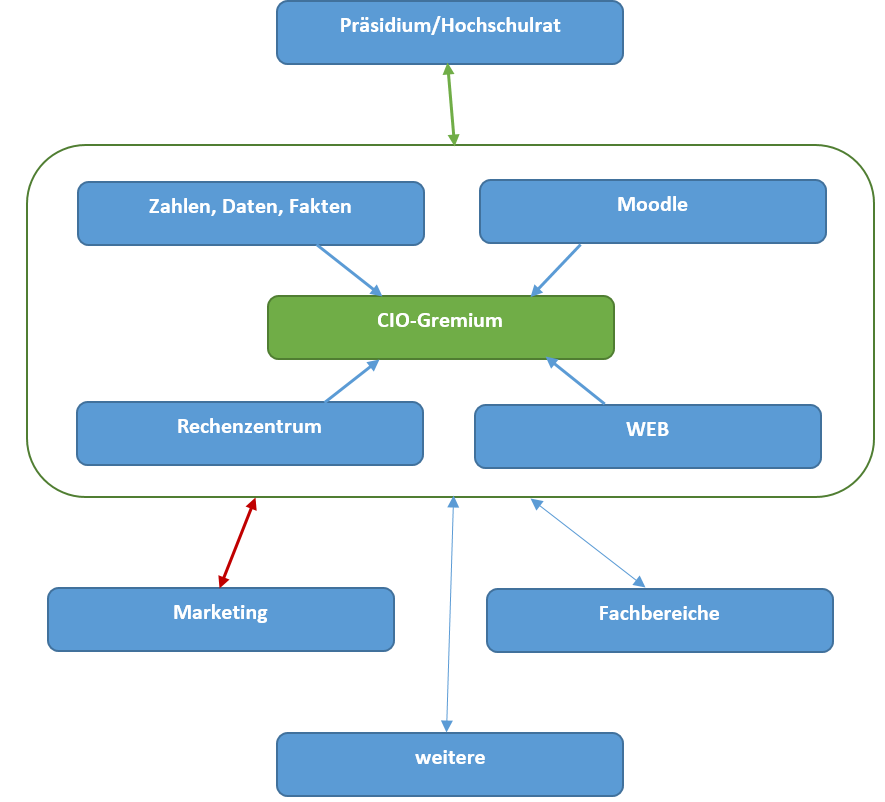
\includegraphics[width=\textwidth]
	{kapitel/gruppe3/bilder/moegliches_cio_gremium}
	\caption{Umstellung/Änderung des Organigramms der Hochschule Emden 	hinsichtlich eines CIO Gremiums}	
	\label{fig_moegliches_gremium}
\end{figure}

In Verbindung mit den drei bereits existierenden Arbeitsgruppen würde sich eine Mischform zwischen strategischem und kollektivem CIO für die Hochschule Emden/Leer anbieten. Das bietet die Möglichkeit sich den gegenebheien der Hochschule anzupassen und ein auf Emden/Leer awäre, dass das CIO-Gremium eng mit dem Marketing zusammenarbeitet und somit von der vorgestellten Möglichkeit Feedback zu sammeln, beschrieben in \ref{feedback} profitieren würde. So können anfallende Probleme direkt diskutiert und Lösungen gefunden werden. 



